\documentclass[a4paper,12pt]{report} %размер бумаги устанавливаем А4, шрифт 12пунктов
\usepackage[T2A]{fontenc}
\usepackage[utf8]{inputenc}%включаем свою кодировку: koi8-r или utf8 в UNIX, cp1251 в Windows
\usepackage{lingmacros}
\usepackage{tree-dvips}
\usepackage[english,russian]{babel}%используем русский и английский языки с переносами
\usepackage{amssymb,amsfonts,amsmath,mathtext,cite,enumerate,float} %подключаем нужные пакеты расширений
\makeatletter
\usepackage[dvips]{graphicx}
\graphicspath{{images/}{images-arch/}}%пути к рисункам

\renewcommand{\@biblabel}[1]{#1.}% Заменяем библиографию с квадратных скобок на точку:
\makeatother
\usepackage{geometry} % Меняем поля страницы
\geometry{left=2cm}% левое поле
\geometry{right=1.5cm}% правое поле
\geometry{top=1cm}% верхнее поле
\geometry{bottom=2cm}% нижнее поле

\renewcommand{\theenumi}{\arabic{enumi}}% Меняем везде перечисления на цифра.цифра
\renewcommand{\labelenumi}{\arabic{enumi}}% Меняем везде перечисления на цифра.цифра
\renewcommand{\theenumii}{.\arabic{enumii}}% Меняем везде перечисления на цифра.цифра
\renewcommand{\labelenumii}{\arabic{enumi}.\arabic{enumii}.}% Меняем везде перечисления на цифра.цифра
\renewcommand{\theenumiii}{.\arabic{enumiii}}% Меняем везде перечисления на цифра.цифра
\renewcommand{\labelenumiii}{\arabic{enumi}.\arabic{enumii}.\arabic{enumiii}.}% Меняем везде перечисления на цифра.цифра

% \arabic{section}

\begin{document}
\begin{titlepage}
\newpage

\begin{center}
ФЕДЕРАЛЬНОЕ АГЕНТСТВО ПО ОБРАЗОВАНИЮ РФ \\
\vspace{1cm}
Н-СКИЙ АРБУЗО-ЛИТЕЙНЫЙ ИНСТИТУТ \\*
(ГОСУДАРСТВЕННЫЙ УНИВЕРСИТЕТ) \\*
\hrulefill
\end{center}

\flushright{КАФЕДРА \No ХХХ}

\vspace{8em}

\begin{center}
\Large Пояснительная записка \\ к дипломному проекту на тему:
\end{center}

\vspace{2.5em}

\begin{center}
\textsc{\textbf{исследование торсионных наногенераторов \linebreak стволовых клеток для борьбы с терроризмом}}
\end{center}

\vspace{6em}

\begin{flushleft}
Студент--дипломник \hrulefill Пупкин А.А. \\
\vspace{1.5em}
Научный руководитель \\
доцент \hrulefill Иванов Б.Б.\\
\vspace{1.5em}
Рецензент \\
к.ф.-м.н., в.н.с. АБВГ \hrulefill Петров В.В.\\
\vspace{1.5em}
Зав. кафедрой \No ХХХ \\
д.ф-м.н, профессор \hrulefill Сидоров Г.Г.
\end{flushleft}

\vspace{\fill}

\begin{center}
Н-ск 2000
\end{center}

\end{titlepage}
% это титульный лист
\tableofcontents % это оглавление, которое генерируется автоматически

\newpage

\chapter*{Введение}
\addcontentsline{toc}{chapter}{Введение}

Данная группавая работа представляет собой программный комплекс для проведения целевой компьютерной экспертизы. \\
В этом семестре было поставлено несколько целей: \\

\begin{enumerate}
\item При разработке использовать систему контроля версий (так как в группе несколько программистов)
\item Документация должна быть составлена в LaTex (при использовании системы контроля версий это дает возможность совместно разрабатывать документацию)
\item Изучение Qt (кросплатформенная и прочее)
\item Создание архитектуры которая позволила бы как объеденить наработки из прошлого семестра, так и дописать новые модули для проведения компьютерной экспертизы
\item Подготовка документации к внедрению
\end{enumerate}% Это введение
% \newpage

\chapter{Архитектура}
% \addcontentsline{toc}{chapter}{Архитектура}

\section{Основной алгоритм}
В ходе разарботки были применены видоизменненный шаблон проектирования: Fabrics. 
Основной алгоритм представлен на рисунке(см. рис.~\ref{ris:alg_main})

\begin{figure}[h]
\center{ 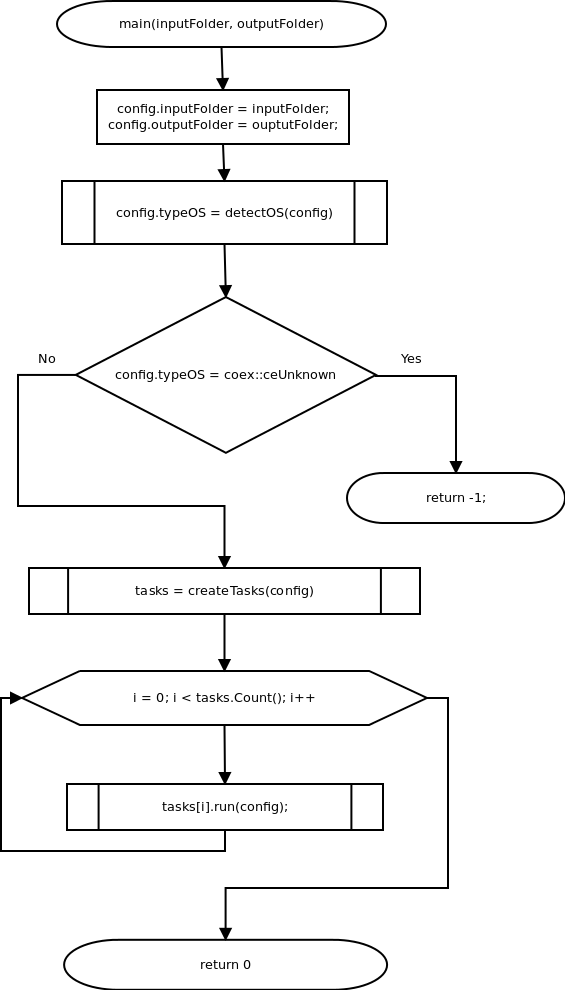
\includegraphics[width=0.5\linewidth]{alg_main} }
\caption{Основной алгоритм.}
\label{ris:alg_main}
\end{figure}
% Про архитектуру



\newpage

\section*{Notes for My Paper}

Don't forget to include examples of topicalization.
They look like this:

{\small
\enumsentence{Topicalization from sentential subject:\\ 
\shortex{7}{a John$_i$ [a & kltukl & [el & 
  {\bf l-}oltoir & er & ngii$_i$ & a Mary]]}
{ & {\bf R-}clear & {\sc comp} & 
  {\bf IR}.{\sc 3s}-love   & P & him & }
{John, (it's) clear that Mary loves (him).}}
}

\subsection*{How to handle topicalization}

I'll just assume a tree structure like (\ex{1}).

{\small
\enumsentence{Structure of A$'$ Projections:\\ [2ex]
\begin{tabular}[t]{cccc}
    & \node{i}{CP}\\ [2ex]
    \node{ii}{Spec} &   &\node{iii}{C$'$}\\ [2ex]
        &\node{iv}{C} & & \node{v}{SAgrP}
\end{tabular}
\nodeconnect{i}{ii}
\nodeconnect{i}{iii}
\nodeconnect{iii}{iv}
\nodeconnect{iii}{v}
}
}

\subsection*{Mood}
какая то хрень

Mood changes when there is a topic, as well as when
there is WH-movement.  \emph{Irrealis} is the mood when
there is a non-subject topic or WH-phrase in Comp.
\emph{Realis} is the mood when there is a subject topic
or WH-phrase.

\end{document}